%% Copernicus Publications Manuscript Preparation Template for LaTeX Submissions
%% ---------------------------------
%% This template should be used for the following class files: copernicus.cls, copernicus2.cls, copernicus_discussions.cls
%% The class files, the Copernicus LaTeX Manual with detailed explanations regarding the comments
%% and some style files are bundled in the Copernicus Latex Package which can be downloaded from the different journal webpages.
%% For further assistance please contact the Publication Production Office (production@copernicus.org).
%% http://publications.copernicus.org


%% Differing comments regarding the specific class files are highlighted.


%% copernicus.cls
\documentclass[acp]{copernicus}

%% copernicus2.cls
%\documentclass[journal abbreviation]{copernicus2}

%% copernicus_discussions.cls
%\documentclass[journal abbreviation, hvmath, online]{copernicus_discussions}


\begin{document}


\title{Something about cloud tracking}


\author[1]{Jordan T Dawe}
\author[1]{Philip H Austin}

\affil[1]{Department of Earth and Ocean Sciences, 
        University of British Columbia, 
	6339 Stores Road, 
        Vancouver, BC, 
        V6T 1Z4}

%% The [] brackets identify the author to the corresponding affiliation, 1, 2, 3, etc. should be inserted.



\runningtitle{CLOUD TRACKING}

\runningauthor{Dawe and Austin}

\correspondence{Jordan T Dawe\\ (jdawe@eos.ubc.ca)}



\received{}
\pubdiscuss{} %% only important for two-stage journals
\revised{}
\accepted{}
\published{}

%% These dates will be inserted by the Publication Production Office during the typesetting process.


\firstpage{1}

\maketitle



\begin{abstract}
A technique for the tracking of individual clouds in an large eddy 
simulation model is presented.
\end{abstract}


%% only used for copernicus2.cls
%\abstract{
% TEXT
% \keywords{TEXT}}



\introduction
%% \introduction[modified heading if necessary]
TEXT



\section{Model Description}

All LES calculations in this paper were made using the System for Atmospheric 
Modeling \citep[SAM;][]{Khairoutdinov2003}.  SAM is an anelastic LES 
Two model runs were performed, 
configured as standard Global Energy and Water Cycle Experiment (GEWEX) 
Cloud System Studies \citep[GCSS;][]{Randall2003} experiments: a Barbados 
Oceanographic and Meteorological Experiment \citep[BOMEX;][]{Siebesma2003} run,
and an Atmospheric Radiation Measurement Study \citep[ARM;][]{Brown2002} run. 

\subsection{BOMEX}

BOMEX simulates a trade-wind cumulus cloud field that was observed over the 
ocean near Bermuda
The BOMEX run was performed on a 6.4 km x 6.4 km horizontal x 3.2 km vertical 
domain with 25 meter grid resolution in all directions for 6 hours, and the 
first three hours of simulation were discarded. 

\subsection{ARM}

The ARM run was performed on a 7.68 km x 7.68 km x 4.5 km domain with 30 meter 
grid resolution.


%==============================================================================

\section{Cloud Tracking}

Dividing a cloud field up into individual clouds at a single moment in time is 
a trivial matter.  Tracking the resulting clouds from one time step to the 
next is much more problematic, as a cloud is not a consistent physical object; 
it is, rather, a series of processes.  A rising parcel of moist air may 
condese, a parcel of air containing condensate may evaporate, and a cloud may 
be split in two by air turbulence or collide with another cloud and merge into 
one.  To be able to handle all of these processes, we adopt a more complex 
definition of what constitutes an individual cloud.

We begin by defining two cloud regions.  First is the cloud core, defined following 
\cite{Siebesma1995} as all cloudy points which have positive buoyancy and 
upward velocity.  Second is the cloud plume, the total region of air that has 
been influenced by the cloud.  We define this region following the work of 
\cite{Couvreaux2010} via a numerical tracer that is emitted at the surface and 
subsequently decays exponentially with a one minute time constant.  A point is 
considered to be in the plume if the tracer value of that point is larger than 
one standard deviation above the mean tracer value at the current model height.
Additionally, the tracer must exceed five precent of the value of the tracer 
standard deviation integrated from the surface to the current height.  Unlike 
Couvreaux et al., however, we do not require these plume points to be moving 
upward or to have condensed liquid water.

In general, the core region is a subset of the plume region.  The purpose of 
these two regions is to determine when a cloud splits and merges: if two cloud 
cores touch, the clouds are considered to have merged, and if parts of a cloud 
seperate such that their plumes no longer touch, the clouds are considered to 
have split.  This definition makes clouds slightly ``sticky'', ensuring that 
clouds do not rapidly split and merge as small tendrils are torn from the main 
cloud mass and evaporate.

Next, we identify the distance of all core grid cells from the core surface--
the "depth" into the cloud mass of the grid cell (Fig. 
\ref{fig:cloudfinder_instructions}a).  We do this by labeling all core grid 
cells directly adjactent to a non-core grid cell with '1'; grid cells 
diagonally adjacent are ignored.  Then core cells adjactent to the cells 
labelled '1' are labelled '2', and the process is repeated until all core grid 
cells are labelled with their depth.

Next, we divide the field up into "cloudlets", sub-units of the core which are 
centered on points that are far from the core surface, using a process based 
on ideas of crystal growth (Fig. \ref{fig:cloudfinder_instructions}b).  First, 
we select one of the deepest points in the core and assign it to a cloudlet.  
Next, any points at the same depth which are touching the cloudlet are absorbed 
into the cloudlet, until the cloudlet is no longer touching unassigned points.  
If there are still points at the same depth they are not part of the cloudlet; 
a new point is selected, assigned to a new cloudlet, and this process is 
repeated until all the deepest grid cells are assigned to cloudlets.  Then the 
next-deepest points are selected, and each cloudlet is expanded into these 
points.  Points that could be assigned to more than one cloudlet go to the 
nearest cloudlet, or are assigned randomly if two cloudlets are equally 
distant.  Points that remain unassigned are added to new cloudlets in the same 
manner as the deepest points, and the process is repeated until all core points 
are assigned to a cloudlet.

Once all the core points have been assigned to cloudlets, this process is 
continued for the plume points in the same manner, until the plume points have 
all been assigned to cloudlets as well.  Note that it is possible to have a 
cloudlet that has no core points.  This process is repeated for every saved 
model time step.

Next, any cloudlets which have spatially connected cores in the first time step 
are joined into clouds.  At subsequent time steps, cloudlets that spatially 
overlap with a cloud at the previous timestep are assumed to be the same cloud.
The cloudlet's position is corrected by calculating the cloudlet's mean 
velocity and the distance the cloudlet would have moved over the time step is 
removed.  If a cloudlet overlaps two or more clouds, the cloudlet is assigned 
to the cloud with the greatest spatial overlap.  Any cloudlets that do not 
overlap clouds in the previous time step are assumed to be new clouds.

At this point merges and splits are performed.  Any clouds that have connected 
cores are merged into a single cloud, with the largest cloud engulfing the 
smaller clouds.  Any cloud which contains cloudlets that do not have connected
plumes are split into two clouds, with the largest sub-cloud being assigned to 
the original cloud and the smaller sub-clouds becoming new clouds.  Then the 
process of cloudlet assignment, merging, and splitting is repeated with the 
next time step, until all cloudlets are assigned to a cloud.

Once the clouds are all assigned, any cloud that is present for less than 
five minutes is flagged as noise and analyzed seperately from the rest of 
the clouds.  The remaining clouds are formed into a network graph, and 
connected subgraphs are assumed to be a single coherent cloud structure.  This 
step is neccessary to handle events where a cloud splits in two, but then 
merges back together at a later time step.

%==============================================================================

\section{Tracked Cloud Statistics}
TEXT

\subsection{BOMEX}
TEXT

\subsection{ARM}
TEXT


\conclusions
%% \conclusions[modified heading if necessary]
TEXT




%\appendix
%\section{\\ \\ \hspace*{-7mm} HEADING}    %% Appendix A

%\subsection                               %% Appendix A1, A2, etc.




\begin{acknowledgements}
Support for this research was provided by the Canadian Foundation for Climate 
and Atmospheric Science through the Cloud Aerosol Feedback and Climate 
network.  Figures were generated using the matplotlib library in the Python
programming language.
\end{acknowledgements}


\bibliographystyle{copernicus}
\bibliography{./bibliography/cloud_tracking}


%% Literature citations
%% command                        & example result
%% \citet{jones90}|               & Jones et al.\ (1990)
%% \citep{jones90}|               & (Jones et al., 1990)
%% \citep{jones90,jones93}|       & (Jones et al., 1990, 1993)
%% \citep[p.~32]{jones90}|        & (Jones et al., 1990, p.~32)
%% \citep[e.g.,][]{jones90}|      & (e.g., Jones et al., 1990)
%% \citep[e.g.,][p.~32]{jones90}| & (e.g., Jones et al., 1990, p.~32)
%% \citeauthor{jones90}|          & Jones et al.
%% \citeyear{jones90}|            & 1990






%% FIGURES %%%%%%%%%%%%%%%%%%%%%%%%%%%%%%%%%%%%%%%%%%%%%%%%%%%%%%%%%%%%%%%%%%%%


%% ONE-COLUMN FIGURES

%f
%\begin{figure}[t]
%\vspace*{2mm}
%\begin{center}
%\includegraphics[width=8.3cm]{./figures/figure1}
%\end{center}
%\caption{Schematic representation of our cloudlet algorithm.}
%\label{fig:cloudfinder_instructions}
%\end{figure}


%% TWO-COLUMN FIGURES

%f
\begin{figure}[t]
\vspace*{2mm}
\begin{center}
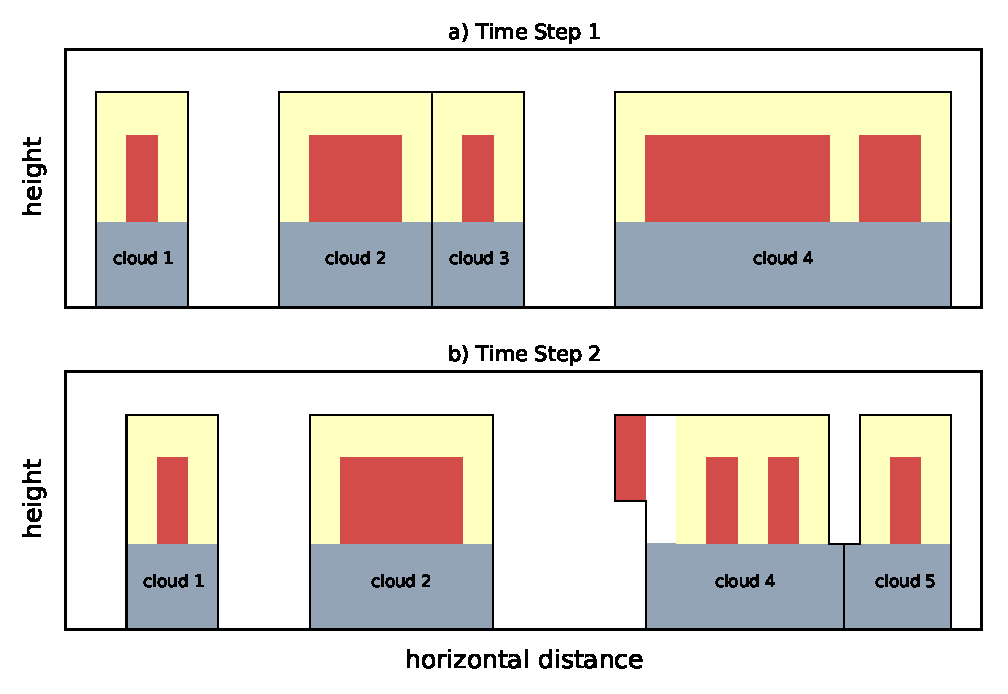
\includegraphics[width=12cm]{./figures/cloudfinder_instructions}
\end{center}
\caption{Schematic representation of our cloud tracking algorithm.}
\label{fig:cloudfinder_instructions}
\end{figure}


%% TABLES %%%%%%%%%%%%%%%%%%%%%%%%%%%%%%%%%%%%%%%%%%%%%%%%%%%%%%%%%%%%%%%%%%%%


%% ONE-COLUMN TABLE

%t
%\begin{table}[t]
%\caption{TEXT}
%\vskip4mm
%\centering
%\begin{tabular}{column = lcr}
%\tophline

%\middlehline

%\bottomhline
%\end{tabular}
%\end{table}


%% TWO-COLUMN TABLE

%t
%\begin{table*}[t]
%\caption{TEXT}
%\vskip4mm
%\centering
%\begin{tabular}{column = lcr}
%\tophline

%\middlehline

%\bottomhline
%\end{tabular}
%\end{table*}


%% The different columns must be seperated with a & command and should
%% end with \\ to identify the column brake.

%%%%%%%%%%%%%%%%%%%%%%%%%%%%%%%%%%%%%%%%%%%%%%%%%%%%%%%%%%%%%%%%%%%%%%%%%%%%%%


%% If figures and tables must be numbered 1a, 1b, etc. the following command
%% should be inserted before the begin{} command.

%\addtocounter{figure}{-1}\renewcommand{\thefigure}{\arabic{figure}a}


\end{document}
